\documentclass[../main.tex]{subfiles}
\graphicspath{{\subfix{../figures/}}}
%
\begin{document}
%
\section{合成模式(Composite)}
合成(Composite)模型模式属于对象的结构模式,有时又叫做部分-整体(Part-Whole)模式。
合成模式将对象组织到树结构中,可以用来描述整体与部分的关系。
合成模式可以使客户端将整体对象与部分对象同等看待。

在下面的情况下应当考虑使用合成模式:
\begin{itemize}
  \item 需要描述对象的部分和整体的等级结构;
  \item 需要客户端忽略掉整体对象和部分对象的区别。
\end{itemize}
%
\textbf{合成模式的典型应用-文件系统}:
一个文件系统就是一个典型的合成模式系统。文件系统是一个树结构。树有节点,节点有两种,一种是树枝节点,即目录,有子树结构;另一种是文件,即树叶节点,没有子树结构。
%
\subsection{对象的树结构}
%
\textbf{有向树结构的分类}:
根据信息传递的方向,有向树结构又可以分为3种,从上向下,从下向上和双向的。
在三种有向树图中,树的节点和他们的相互关系都是一样的,但是连接他们的关系的方向却不同。

\textbf{由上向下的树图}:
在由上向下的树图中,每一个树枝节点都有箭头指向它的所有的子节点,从而一个客户端可以要求一个树枝节点给出所有的子节点,而一个节点却不知道它父节点。在这样的树结构上,信息可以按照箭头所指的方向自上向下传播。
%
\begin{figure}[H]
  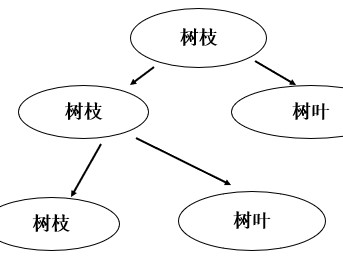
\includegraphics[width=0.30\textwidth]{21_1.jpg}
  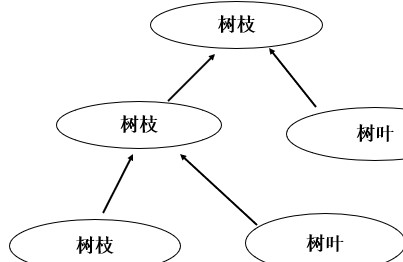
\includegraphics[width=0.30\textwidth]{21_2.jpg}
  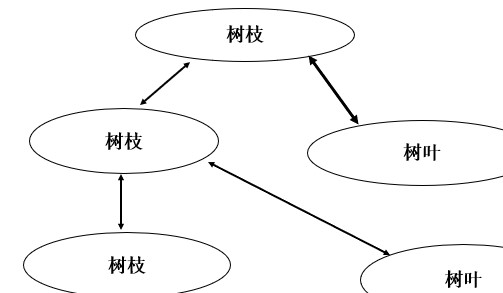
\includegraphics[width=0.30\textwidth]{21_3.jpg}
\end{figure}
%
\textbf{由下向上的树图}:
在一个由下向上的树图中,每一个节点都有箭头指向它的父节点,但是父节点却不知道其子节点。信息可以按照箭头所指的方向自下向上传播。

\textbf{双向的树图}:
在一个双向的树图中,每一个节点都同时知道它的父节点和所有的子节点。在这样的树结构上,信息可以按照箭头所指的方向向两个方向传播。

\textbf{树图中的两种节点}:
一个树结构由2种节点组成:树枝节点和树叶节点。树枝节点可以有子节点,树叶节点不可以有子节点。
注意一个树枝子节点可以不带任何叶子,但是它因为有带有叶子的能力,因此仍然是树枝节点而不会成为叶子节点。
一个树叶节点则永远不可能带有子节点。

\textbf{根节点}:
一个树结构中总有至少一个节点是特殊的节点,称为根节点。一个根节点没有父节点,因为它是树结构的根。
一个树的根节点一般是树枝节点,如果根节点是树叶节点的话,这个树就变成了只有这一个节点的树。

\textbf{树结构的类图}:可以使用类图描述一个树结构的静态结构。下图所示的是合成模式的简略类图,同时也是一个典型的树结构的类图。
\begin{figure}[H]
  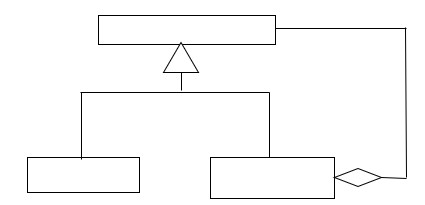
\includegraphics[width=0.25\textwidth]{21_4.jpg}
  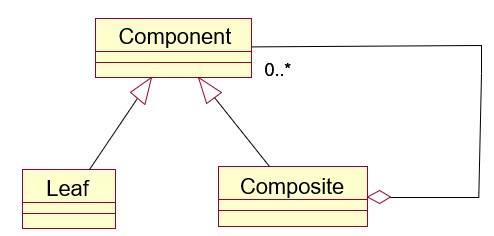
\includegraphics[width=0.45\textwidth]{21_5.jpg}
\end{figure}
%
可看出上面的类图结构涉及到三个角色:
\begin{itemize}
  \item 抽象构件(Component)角色:这是一个抽象角色,它给参加组合的对象规定一个接口。这个角色给出共有的接口及其默认行为。
  \item 树叶构件(Leaf)角色:代表参加组合的树叶对象。一个树叶没有下级的子对象。定义出参加组合的原始对象的行为。
  \item 树枝构件(Composite)角色:代表参加组合的所有包含子对象的对象,并给出树枝构件对象的行为。
\end{itemize}
%
\subsection{合成模式的两种形式}
\textbf{透明方式}:
作为第一种选择,在Component里面声明所有的用来管理子类对象的方法,
包括add()、remove()以及getChild()方法。
好处是所有的构件类都有相同的接口。缺点是不够安全,因为树叶类对象和合成类对象在本质上是有区别的。
树叶类对象不可能有下一个层次的对象,因此add()、remove()以及getCHild()是没有意义的,
但编译时期不会出错,只在运行时期才可能会出错。

\textbf{安全方式}:
第二种选择是在Composite类里面声明所有的用来管理子类对象的方法。这样的做法是安全的做法。
这个选择的缺点是不够透明,因为树叶类和合成类将具有不同的接口。

\textbf{安全式的合成模式的结构}:
安全式的合成模式要求管理聚集的方法只出现在树枝构件类中,而不出现在树叶构件类中。其类图如下:
\begin{figure}[H]
  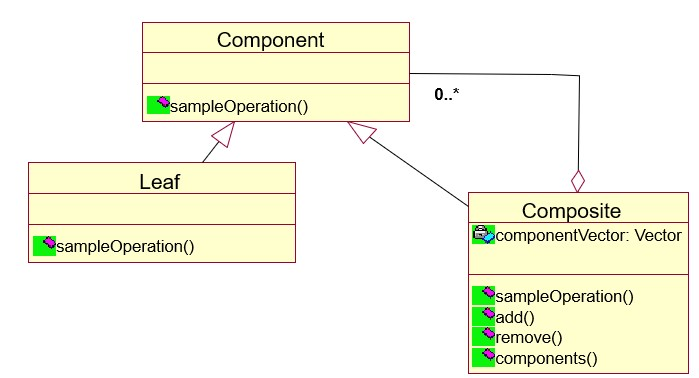
\includegraphics[width=0.75\textwidth]{21_6.jpg}
\end{figure}
%
\begin{lstlisting}[language=java]
import java.util.Vector;
import java.util.Enumeration;
public interface Component {
  Composite getComposite();  // 返返自己的实例
  void sampleOperation();  // 某个业务逻辑方法
}
public class Composite implements Component {
  private Vector componentVector=new java.util.Vector();
  public Composite getComposite() {
    return this; /* 返还自己的实例 */
  }
  public void sampleOperation { /* 某业务逻辑方法 */
   Enumeration enumeration=components();
    while (enumeration.hasMoreElements()) {
      ((Component)enumeration.nextElement()).sampleOperation();
    }
  }
  /* 聚集管理方法,增加一个子构件 */
  public void add(Component component) {
    componentVector.addElement(component);
  }
  /* 聚集管理方法,删除一个子构件 */
  public void remove(Component component) {
    componentVector.removeElement(component);
  }
}
public class Leaf implements Component {
  /* 某业务逻辑方法  */
  public void sampleOperation {  }
  public Composite getComposite() { /* 返还自己的实例 */
    // write your code here
    return null;
  }
}
\end{lstlisting}
%
\textbf{透明式的合成模式的结构}:
透明式的合成模式要求所有的具体构件类,不论是树枝还是树叶,均符合一个统一的接口。其示意类图如下:
\begin{figure}[H]
  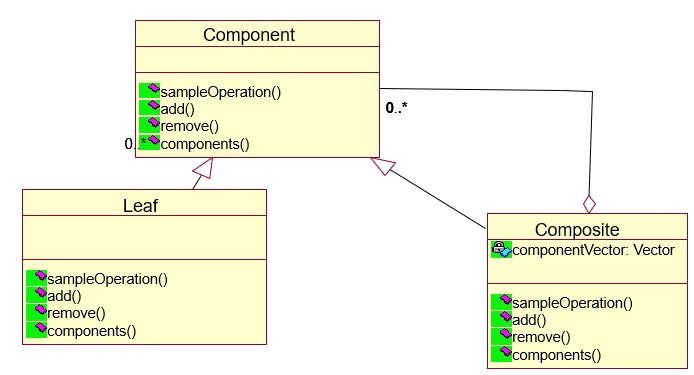
\includegraphics[width=0.75\textwidth]{21_7.jpg}
\end{figure}
%
\begin{lstlisting}[language=java]
import java.util.Vector;
import java.util.Enumeration;
public interface Component {
  Composite getComposite(); // 返返自己的实例
  void sampleoperation();  // 某个业务逻辑方法
  /* 聚集管理方法,增加一个子构件 */
  void add(Component component);
  /* 聚集管理方法,删除一个子构件 */
  void remove(Component component);
  /* 聚集管理方法,返还聚集的Enumeration对象 */
  Enumeration components( );
}
public class Composite implements Component {
  private Vector componentVector=new java.util.Vector();
  public Composite getComposite() { /* 返还自己的实例 */
    return this;
  }
  public void sampleOperation { /* 某业务逻辑方法  */
   Enumeration enumeration=components();
    while (enumeration.hasMoreElements()) {
      ((Component)enumeration.nextElement()).sampleOperation();
    }
  }
  /* 聚集管理方法,增加一个子构件 */
  public void add(Component component) {
    componentVector.addElement(component);
  }
  /* 聚集管理方法,删除一个子构件 */
  public void remove(Component component) {
    componentVector.removeElement(component);
  }
  /* 聚集管理方法,返回聚集的Enumeration对象
  public  Enumeration components() {
    return componentVector.elements();
  }
}
public class Leaf implements Component {
  public void sampleOperation { /* 某个业务逻辑方法  */
    //write your code here
  }
  public Composite getComposite() { /* 返还自己的实例 */
    return null;
  }
  /* 聚集管理方法,增加一个子构件 */
  public void add(Component component) {}
  /* 聚集管理方法,删除一个子构件 */
  public void remove(Component component){}
  /* 聚集管理方法,返回聚集的Enumeration对象 */
  public Enumeration components() { return null; }
}
\end{lstlisting}
%
\textbf{一个绘图的例子}:以一个绘图软件说明合成模式的应用。一个绘图系统给出各种工具用来描绘由线、长方形和圆形等基本图形组成的图形。一个复合的图形是由这些基本图形组成,可以运用合成模式。
合成图形应当有一个列表,存储对所有基本图形的引用。复合图形的draw()方法在调用时,应当逐一调用所有列表上的基本图形的draw()方法。
可以使用两种合成模式来实现:安全式和透明式。
%
\subsection{应用安全式合成模式}
安全式的合成模式意味着只有树枝构件才配有管理聚集的方法,而树叶则没有这些方法。下图所示是使用安全式的设计结构图
\begin{figure}[H]
  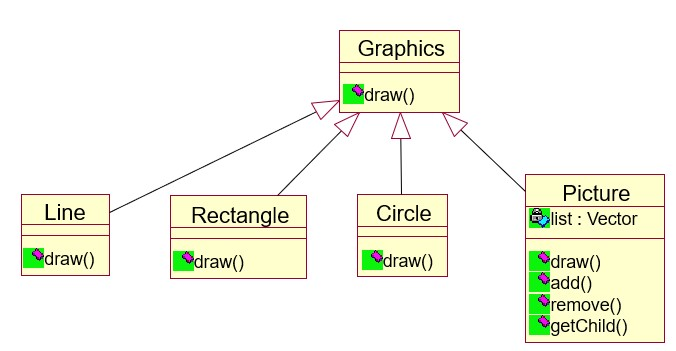
\includegraphics[width=0.75\textwidth]{21_8.jpg}
\end{figure}
%
客户端可以调用add()方法加入一个基本图形,remove()方法取消一个基本图形,getChild(index x)得到组成复杂图形的第x个基本图形。
\begin{lstlisting}[language=java]
// 构件角色Graphics
package com.javapatterns.composite.drawingsafe;
public abstract class Graphics {
  public abstract void draw();
}
// Picture类是树枝构件角色,它实现了抽象构件角色所要求的方法,
// 还额外提供了用于管理子对象聚集的一系列方法
package com.javapatterns.composite.drawingsafe;
import java.util.Vector;
public class Picture extends Graphics {
  private Vector list=new Vector(10);
  public void draw() {
    for (int i=0; i< list.size(); i++) {
      Graphics g = (Graphics)list.get(i);
      g.draw();
    }
  }
  public void add(Graphics g) { /* 聚集管理方法,增加一个子构件 */
    list.add(g);
  }
  public void remove(Graphics g) { /* 聚集管理方法,删除一个子构件 */
    list.remove(g);
  }
  public void getChild(int i) {
    return (Graphics)list.get(i); /* 返还一个子构件 */
  }
}
//Line是树叶构件,它没有任何的子对象,
//因此不必提供管理子对象聚集的方法
package com.javapatterns.composite.drawingsafe;
public class Line extends Graphics {
  public void draw() {
    //write your code
  }
}
//树叶Rectangle
package com.javapatterns.composite.drawingsafe;
public class Rectangle extends Graphics {
  public void draw() {
    //write your code
  }
}
//树叶Circle
package com.javapatterns.composite.drawingsafe;
public class Circle extends Graphics {
  public void draw() {
    //write your code
  }
}
\end{lstlisting}
%
\subsection{应用透明式的合成模式}
透明式合成模式无论树枝和树叶都有管理聚集的方法。其设计图如下:
%
\begin{figure}[H]
  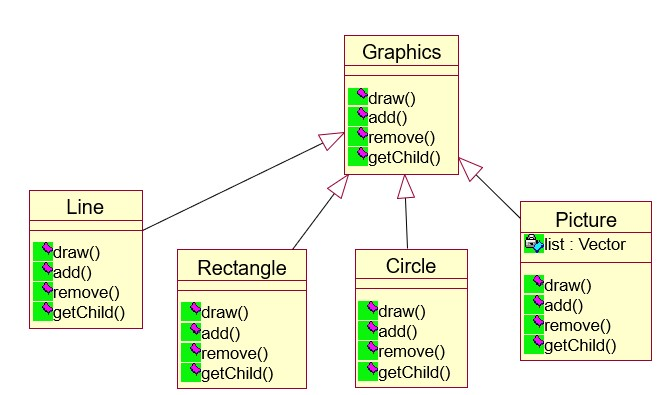
\includegraphics[width=0.75\textwidth]{21_9.jpg}
\end{figure}
%
\begin{lstlisting}[language=java]
// 构件角色Graphics
package com.javapatterns.composite.drawingtransparent;
abstract public class Graphics {
   public abstract void draw();
   public void add(Graphics g); /* 聚集管理方法,增加一个子构件 */
   public void remove(Graphics g); /* 聚集管理方法,删除一个子构件 */
   public Graphics getChild(int i); /* 返还一个子构件 */
}
// Picture类是树枝构件角色,它实现了抽象构件角色所要求的方法,
// 还额外提供了用于管理子对象聚集的一系列方法
package com.javapatterns.composite.drawingtransparent;
import java.util.Vector;
public class Picture extends Graphics {
  private Vector list=new Vector(10);
  public void draw() {
    for (int i=0;i< list.size();i++) {
      Graphics g=(Graphics)list.get(i);
      g.draw();
    }
  }
  /* 聚集管理方法,增加一个子构件 */
  public void add(Graphics g) { list.add(g); }
  /* 聚集管理方法,删除一个子构件 */
   public void remove(Graphics g) { list.remove(g); }
  /* 返还一个子构件 */
   public Graphics getChild(int i) { return (Graphics)list.get(i); }
}
// Line是树叶构件,它必需实现抽象构件角色所要求的方法
package com.javapatterns.composite.drawingtransparent;
public class Line extends Graphics {
  public void draw() {
    //write your code
  }
  /* 聚集管理方法,增加一个子构件 */
  public void add(Graphics g) {
    //do nothing
  }
  /* 聚集管理方法,删除一个子构件 */
  public void remove(Graphics g) {
    //do nothing
  }
  /* 返还一个子构件 */
  public Graphics getChild(int i) { return null; }
}
// Rectangle是树叶构件,它必需实现抽象构件角色所要求的方法
package com.javapatterns.composite.drawingtransparent;
public class Rectangle extends Graphics {
  public void draw() {
    //write your code
  }
  public void add(Graphics g) { // 聚集管理方法,增加一个子构件
    //do nothing
  }
  /* 聚集管理方法,删除一个子构件 */
  public void remove(Graphics g) {
    //do nothing
  }
  /* 返还一个子构件 */
  public void getChild(int i) { return null; }
}
// Circle是树叶构件,它必需实现抽象构件角色所要求的方法
package com.javapatterns.composite.drawingtransparent;
public class Circle extends Graphics {
  public void draw() {
    //write your code
  }
  public void add(Graphics g) { // 聚集管理方法,增加一子构件
    //do nothing
  }
  public void remove(Graphics g) { // 聚集管理方法,删除一个子构件
    //do nothing
  }
  public void getChild(int i) { // 返还一个子构件
    return null;
  }
}
\end{lstlisting}
%
\end{document}
